\documentclass[article,shortnames]{jss}\usepackage[]{graphicx}\usepackage[]{color}
%% maxwidth is the original width if it is less than linewidth
%% otherwise use linewidth (to make sure the graphics do not exceed the margin)
\makeatletter
\def\maxwidth{ %
  \ifdim\Gin@nat@width>\linewidth
    \linewidth
  \else
    \Gin@nat@width
  \fi
}
\makeatother

\definecolor{fgcolor}{rgb}{0.345, 0.345, 0.345}
\newcommand{\hlnum}[1]{\textcolor[rgb]{0.686,0.059,0.569}{#1}}%
\newcommand{\hlstr}[1]{\textcolor[rgb]{0.192,0.494,0.8}{#1}}%
\newcommand{\hlcom}[1]{\textcolor[rgb]{0.678,0.584,0.686}{\textit{#1}}}%
\newcommand{\hlopt}[1]{\textcolor[rgb]{0,0,0}{#1}}%
\newcommand{\hlstd}[1]{\textcolor[rgb]{0.345,0.345,0.345}{#1}}%
\newcommand{\hlkwa}[1]{\textcolor[rgb]{0.161,0.373,0.58}{\textbf{#1}}}%
\newcommand{\hlkwb}[1]{\textcolor[rgb]{0.69,0.353,0.396}{#1}}%
\newcommand{\hlkwc}[1]{\textcolor[rgb]{0.333,0.667,0.333}{#1}}%
\newcommand{\hlkwd}[1]{\textcolor[rgb]{0.737,0.353,0.396}{\textbf{#1}}}%

\usepackage{framed}
\makeatletter
\newenvironment{kframe}{%
 \def\at@end@of@kframe{}%
 \ifinner\ifhmode%
  \def\at@end@of@kframe{\end{minipage}}%
  \begin{minipage}{\columnwidth}%
 \fi\fi%
 \def\FrameCommand##1{\hskip\@totalleftmargin \hskip-\fboxsep
 \colorbox{shadecolor}{##1}\hskip-\fboxsep
     % There is no \\@totalrightmargin, so:
     \hskip-\linewidth \hskip-\@totalleftmargin \hskip\columnwidth}%
 \MakeFramed {\advance\hsize-\width
   \@totalleftmargin\z@ \linewidth\hsize
   \@setminipage}}%
 {\par\unskip\endMakeFramed%
 \at@end@of@kframe}
\makeatother

\definecolor{shadecolor}{rgb}{.97, .97, .97}
\definecolor{messagecolor}{rgb}{0, 0, 0}
\definecolor{warningcolor}{rgb}{1, 0, 1}
\definecolor{errorcolor}{rgb}{1, 0, 0}
\newenvironment{knitrout}{}{} % an empty environment to be redefined in TeX

\usepackage{alltt}

\usepackage{acronym}
\usepackage{cleveref}
\usepackage{subfig}

\acrodef{CRAN}[CRAN]{Comprehensive \proglang{R} Archive Network}
\acrodef{mlp}[MLP]{multilayer perceptron}
\acrodef{nid}[NID]{neural interpretation diagram}

%%%%%%%%%%%%%%%%%%%%%%%%%%%%%%
%% declarations for jss.cls %%%%%%%%%%%%%%%%%%%%%%%%%%%%%%%%%%%%%%%%%%
%%%%%%%%%%%%%%%%%%%%%%%%%%%%%%

%% almost as usual
\author{Marcus W. Beck\\Oak Ridge Institute for Science and Education\\US Environmental Protection Agency}
\title{\pkg{NeuralNetTools}: Visualization and Analysis Tools for Neural Networks}

%% for pretty printing and a nice hypersummary also set:
\Plainauthor{Marcus W. Beck} %% comma-separated
\Plaintitle{NeuralNetTools: Visualization and Analysis Tools for Neural Networks} %% without formatting
\Shorttitle{\pkg{NeuralNetTools}: Visualization and Analysis Tools for Neural Networks} 

%% an abstract and keywords
\Abstract{
Functions within this package can be used for the interpretation of neural network models created in \proglang{R}, including functions to plot a neural network interpretation diagram, evaluation of variable importance, and a sensitivity analysis of input variables.
}
\Keywords{neural networks, plotnet, sensitivity, variable importance, \proglang{R}}
\Plainkeywords{neural networks, plotnet, sensitivity, variable importance, R} %% without formatting
%% at least one keyword must be supplied

%% publication information
%% NOTE: Typically, this can be left commented and will be filled out by the technical editor
%% \Volume{50}
%% \Issue{9}
%% \Month{June}
%% \Year{2012}
%% \Submitdate{2012-06-04}
%% \Acceptdate{2012-06-04}

%% The address of (at least) one author should be given
%% in the following format:
\Address{
  Marcus W. Beck\\
  Oak Ridge Institude for Science and Education\\
  US Environmental Protection Agency\\
  National Health and Environmental Effects Research Laboratory\\
  Gulf Ecology Division, 1 Sabine Island Drive\\
  Gulf Breeze, Florida, 32561, USA\\
  E-mail: \email{beck.marcus@epa.gov}
}
%% It is also possible to add a telephone and fax number
%% before the e-mail in the following format:
%% Telephone: +43/512/507-7103
%% Fax: +43/512/507-2851

% knitr options

% get online bib file


%% need no \usepackage{Sweave.sty}
\IfFileExists{upquote.sty}{\usepackage{upquote}}{}
\begin{document}

%% Note that you should use the \pkg{}, \proglang{} and \code{} commands.

\section[Introduction]{Introduction}

Data science is a relatively new paradigm of analysis that focuses on the synthesis of unstructured information from multiple sources to identify patterns or trends `born from the data' \citep{Kelling09}.  A central theme is the focus on data exploration and prediction as compared to hypothesis-testing using domain-specific methods for scientific exploration \citep{Kell03}.  Demand for quantitative toolsets to address challenges in data-rich environments has increased drastically with the advancement of techniques for rapid acquisition of data. Fields of research characterized by high-throughput data have a strong foundation in computationally-intensive methods of analysis (e.g., \citet{Saeys07}).  Morever, disciplines that have historically been limited by data quantity, such as ecological studies across broad temporal and spatial scales, have also realized the importance of data intensive approaches given the increasing use of novel techniques to acquire information (e.g., \citet{Swanson15}).  Regardless of the discipline, quantitative methods that explicitly focus on inductive reasoning can serve a complementary role to conventional, hypothesis-driven approaches to scientific discovery \citep{Kell03}.  

Statistical methods that have been used to support data exploration for inductive analysis are numerous \citep{Jain00}.  A common theme among these methods is the use of machine-learning algorithms where the primary objective is to identify emergent patterns in the data with minimal human intervention.  Neural networks, in particular, are designed to mimic the neuronal structure of the human brain by `learning' inherent data structures through adaptive algorithms \citep{Rumelhart86,Ripley96}.  Although the conceptual model was introduced several decades ago \citep{McCulloch43}, neural networks have had a central role in data intensive science.  The most popular form of neural network is the feed-forward \ac{mlp} trained using the backpropagation algorithm \citep{Rumelhart86}.  This model is typically used to predict the response of one or more variables given one to many explanatory variables.  The hallmark feature of the \ac{mlp} is the characterization of relationships using an arbitrary number of parameters (i.e., the hidden layer) that are chosen through an iterative training process with the backpropation algorithm.  Conceptually, the \ac{mlp} is nothing more than a hyper-parameterized non-linear model that can fit a smooth function to any dataset with almost non-existent residual error \citep{Hornik91}.

An arbitrarily large number of parameters to fit a neural network provides obvious predictive advantages, but conversely complicates the extraction of critical model information.  Information such as variable importance or model sensitivity are necessary aspects of exploratory data analysis that are not easily obtained from a neural network. As such, a common criticism is that neural networks are `black-boxes' that offer minimal insight into relationships among variables \citep[e.g.,][]{Paruelo97}.  \citet{Olden02} provide a rebuttal to this concern by describing methods to extract information from neural networks, most of which were previously available but not commonly used.  For example, \citet{Olden02} describe  the \ac{nid} for plotting \citep{Ozesmi99}, the Garson algorithm for variable importance \citep{Garson91}, and the Profile method for sensitivity analysis \citep{Lek96}.  These quantitative tools `illuminate the black box' by disaggregating the network parameters to characterize relationships between variables that are described by the model.  In essence, \ac{mlp} neural networks were developed for prediction but methods described in \citep{Olden02} leverage these models to describe data signals.  Increasing the accesibility of these diagnostic tools will have value for exploratory analysis in data science.

This article describes the \pkg{NeuralNetTools} package for \proglang{R} that was developed to improve the breadth and quality of information obtained from the \ac{mlp} neural network.  Functions provided by the package are those previously described in \citep{Olden02} but have not been available in an open-source programming environment.  The reach of the package is all-inclusive such that generic functions were developed using S3 methods for all neural network object classes available in \proglang{R}.  The objecives of this article are to 1) provide an overview of the statistical foundation the \ac{mlp} network, 2) briefly describe similarities and differences between existing neural network packages in \proglang{R}, and 3) describe the theory and application of the primary functions in the \pkg{NeuralNetTools} package.  The package is currently available on the \ac{CRAN}, whereas the development version is maintained as a GitHub repository.  

\section[Theoretical foundation]{Theoretical foundation and existing R packages}

An intriguing characteristic of neural networks is the relaxation of assumptions for the distributional characteristics of the response variables.  Unlike conventional approaches, neural networks have been popularized by their ability to model response variables with arbitrary distributions and can describe relationships in datasets with noisy or imprecise information.  The typical \ac{mlp} network is composed of multiple layers that define the transfer of information between input and response layers.  Information travels in one direction where a set of values for one to many variables in the input layer propagates through one or more hidden layers to the resulting layer of the response variables. `Hidden' layers between the input and response layers are key components of a neural network that mediate the transfer of information.  Just as the input and response layers are composed of variables or `nodes', each hidden layer is composed of nodes with weighted connections that define the strength of information flow between layers.  `Bias' layers connected to hidden and response layers may also be used that are analagous to intercept terms in a standard regression model.

Training a neural network model requires identifying the `optimal' weights that define the connections between the model layers.  The optimal weights are those that minimize prediction error for a test dataset that is independent of the training dataset.  Training is commonly achieved using the backpropagation algorithm described in detail in \citep{Rumelhart86}.  This algorithm identifies the optimal weighting scheme between layers through an iterative process where weights are gradually changed through a forward- and backward-propagation process \citep{Rumelhart86,Lek00}.  The algorithm begins by assigning an arbitrary weighting scheme to the connections in the network, followed by estimating the output in the response variable through the forward-propagation of information through the network, and finally calculating the difference between the predicted and actual value of the response.  The weights are then changed through a back-propagation step that begins by changing weights in the output layer and then the remaining hidden layers.  The process is repeated until the chosen error function is minimized.  Formulaically, a generic \ac{mlp} neural network can be represented as \citep{Ripley96}:
\begin{equation}
y_k = f_k \left(\sum\limits_{j=1}^k w_{jk}f_j \left( \sum\limits_{i=1}^j w_{ij}x_i\right) \right)
\end{equation}
where the estimated value of the response variable $y_k$ is a summation of the product between multiple input variables $x$ and multiple hidden nodes $j$, as mediated by the respective weights $w$ and activation functions $f_j$ and $f_k$ for each hidden and output node as the information progresses through the network.



Methods in \pkg{NeuralNetTools} were written for several \proglang{R} packages that can be used to create \ac{mlp} neural networks: \pkg{neuralnet} \citep{Fritsch12}, \pkg{nnet} \citep{Venables02}, and \pkg{RSNNS} \citep{Bergmeir12}. Limited methods were also developed for neural network objects created with the \code{train} function from the \pkg{caret} package \citep{Kuhn15}.  Additional \proglang{R} packages that can create \ac{mlp} neural networks include \pkg{AMORE} that implements the ``TAO-robust back-propagation algorithm'' for model fitting \citep{Castejon14}, \pkg{FCNN4R} as an \proglang{R} interface to the \pkg{FCNN} \proglang{C++} library \citep{Klima15}, \pkg{monmlp} for networks with partial monotonicity constraints \citep{Cannon15}, and \pkg{qrnn} for quantile regression neural networks \citep{Cannon11}.  At the time of writing, the \ac{CRAN} download logs \citep{Csardi15} showed that the \proglang{R} packages with methods in \pkg{NeuralNetTools} included 94\% of all downloads for the available \ac{mlp} packages, with \pkg{nnet} accounting for over 78\%.  As such, methods have not been included in \pkg{NeuralNetTools} for the remaining packages, although further development of \pkg{NeuralNetTools} could include additional methods based on popularity.  Methods are currently available for  \code{mlp} (\pkg{RSNNS}), \code{nn} (\pkg{neuralnet}), \code{nnet} (\pkg{nnet}), and \code{train} (\pkg{caret}, only if the object also inherits from the \code{nnet} class) objects.  Additional \code{default} or \code{numeric} methods are available for some of the generic functions.

\section[Package structure]{Package structure}

The stable release of \pkg{NeurelNetTools} can be installed from \ac{CRAN} and the development version can be installed from GitHub:

\begin{kframe}
\begin{alltt}
\hlcom{# install from CRAN}
\hlkwd{install.packages}\hlstd{(}\hlstr{'NeuralNetTools'}\hlstd{)}
\hlkwd{library}\hlstd{(NeuralNetTools)}

\hlcom{# install from GitHub}
\hlkwd{install.package}\hlstd{(}\hlstr{'devtools'}\hlstd{)}
\hlkwd{library}\hlstd{(devtools)}
\hlkwd{install_github}\hlstd{(}\hlstr{'fawda123/NeuralNetTools'}\hlstd{)}
\hlkwd{library}\hlstd{(NeuralNetTools)}
\end{alltt}
\end{kframe}

\pkg{NeuralNetTools} includes four main functions that were developed following techniques described in \citet{Olden02} and references therein.  These functions include \code{plotnet} to plot a neural network interpretation diagram, \code{garson} and \code{olden} functions to evaluate variable importance, and \code{lekprofile} for a sensitivity analysis of neural network response to input variables.  Most of the functions require the extraction of model weights in a common format for each of the neural network object classes in \proglang{R}.  The \code{neuralweights} function can be used to retrieve model weights for any of the model classes describe above.  A two-element \code{list} is returned with the first element describing the structure of the network and the second element as a named list of weight values for the input model.  The function is used internally within the main package functions but may be useful for comparing networks of different object classes.

A sample dataset is also included with \pkg{NeuralNetTools}.  The \code{neuraldat} dataset is a simple \code{data.frame} with 2000 rows of observations and columns for two response variables (\code{Y1} and \code{Y2}) and three input variables (\code{X1}, \code{X2}, and \code{X3}.  The input variables are random observations from a standard normal distribution and the response variables are linear combinations of the input variables with additional random components.  The response variables are also standardized from zero to one.  A common approach for data preprocessing prior to creating a neural network is to normalize the input variables and to standardize the response variables \citep{Lek00,Olden02}.  Novel datasets can be preprocessed to this common format using the \code{scale} function from \pkg{base} and the \code{rescale} function from \pkg{scales} for the input and response variables, respectively.  The examples below use three models created from the \code{neuraldat} dataset and include \code{mlp} (\pkg{RSNNS}), \code{nn} (\pkg{RSNNS}), and \code{nnet} (\pkg{nnet}) objects (note the syntax differences).


\begin{knitrout}
\definecolor{shadecolor}{rgb}{0.969, 0.969, 0.969}\color{fgcolor}\begin{kframe}
\begin{alltt}
\hlcom{# set random seed for initial weights for training}
\hlkwd{set.seed}\hlstd{(}\hlnum{123}\hlstd{)}

\hlcom{# mlp object, RSNNS package}
\hlkwd{library}\hlstd{(RSNNS)}
\hlstd{x} \hlkwb{<-} \hlstd{neuraldat[,} \hlkwd{c}\hlstd{(}\hlstr{'X1'}\hlstd{,} \hlstr{'X2'}\hlstd{,} \hlstr{'X3'}\hlstd{)]}
\hlstd{y} \hlkwb{<-} \hlstd{neuraldat[,} \hlstr{'Y1'}\hlstd{]}
\hlstd{mod1} \hlkwb{<-} \hlkwd{mlp}\hlstd{(x, y,} \hlkwc{size} \hlstd{=} \hlnum{5}\hlstd{)}

\hlcom{# nn object, neuralnet package}
\hlkwd{library}\hlstd{(neuralnet)}
\hlstd{mod2} \hlkwb{<-} \hlkwd{neuralnet}\hlstd{(Y1} \hlopt{~} \hlstd{X1} \hlopt{+} \hlstd{X2} \hlopt{+} \hlstd{X3,} \hlkwc{data} \hlstd{= neuraldat,} \hlkwc{hidden} \hlstd{=} \hlnum{5}\hlstd{)}

\hlcom{#nnet object, nnet package}
\hlkwd{library}\hlstd{(nnet)}
\hlstd{mod3} \hlkwb{<-} \hlkwd{nnet}\hlstd{(Y1} \hlopt{~} \hlstd{X1} \hlopt{+} \hlstd{X2} \hlopt{+} \hlstd{X3,} \hlkwc{data} \hlstd{= neuraldat,} \hlkwc{size} \hlstd{=} \hlnum{5}\hlstd{)}
\end{alltt}
\end{kframe}
\end{knitrout}

\subsection{Visualizing neural networks}

The number of existing functions in \pkg{R} to view neural networks is minimal.  Such tools have practical use for visualizing network architecture and connections between layers that mediate variable importance. To our knowledge, only the \pkg{neuralnet} and \pkg{FCNN4R} packages provide plotting methods for \ac{mlp} networks in R.  Although useful for viewing the basic structure, the output is minimal and does not include extensive options for customization.

Tbe \code{plotnet} function in \pkg{NeuralNetTools} plots a network as a \acl{nid} \citep{Ozesmi99} and includes several options to customize plot aesthetics. A \ac{nid} is a modification to the standard conceptual illustration of the \ac{mlp} network that allows the user to view the thickness and color of the weight connections based on mangnitude and sign, respectively.  The default settings plot positive weights between layers as black lines and negative weights as grey lines. Line thickness is in proportion to absolute magnitude of each weight (\cref{fig:plotnet}).

\begin{kframe}
\begin{alltt}
\hlkwd{par}\hlstd{(}\hlkwc{mar} \hlstd{=} \hlkwd{c}\hlstd{(}\hlnum{0}\hlstd{,} \hlnum{0}\hlstd{,} \hlnum{0}\hlstd{,} \hlnum{0}\hlstd{))}
\hlkwd{plotnet}\hlstd{(mod3,} \hlkwc{nid} \hlstd{= F,} \hlkwc{circle_col} \hlstd{=} \hlstr{'grey'}\hlstd{,} \hlkwc{bord_col} \hlstd{=} \hlstr{'grey'}\hlstd{)}
\hlkwd{plotnet}\hlstd{(mod3)}
\end{alltt}
\end{kframe}\begin{figure}[!ht]

{\centering \subfloat[\label{fig:plotnet1}]{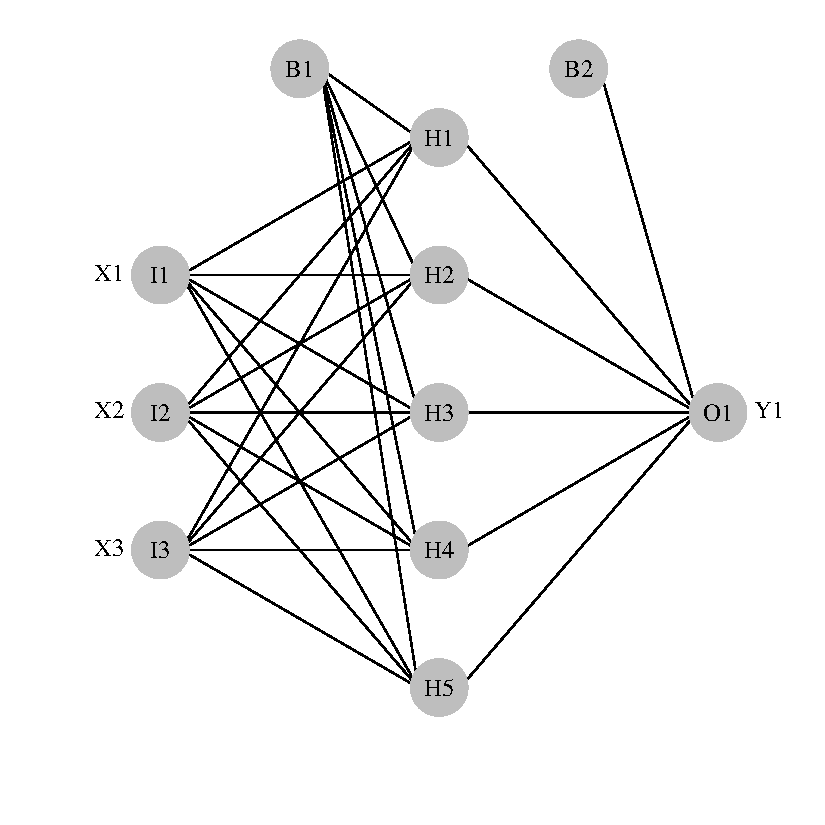
\includegraphics[width=7.5cm,height=7.5cm]{figs/plotnet-1} }
\subfloat[\label{fig:plotnet2}]{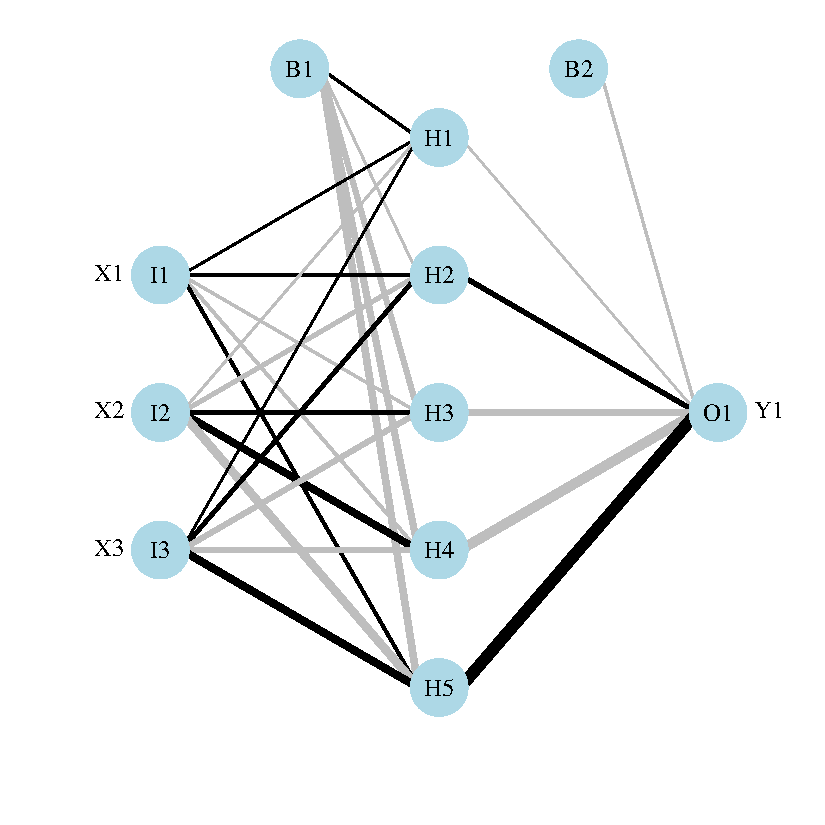
\includegraphics[width=7.5cm,height=7.5cm]{figs/plotnet-2} }

}

\caption{Examples from the \code{plotnet} function showing neural networks as a standard graphic (\ref{fig:plotnet1}) and using the \acl{nid} (\ref{fig:plotnet2}).  Labels outside of the nodes represent variable names and labels within the nodes indicate the layer and node (I: input, H: hidden, O: output, B: bias).  Default options are changed for the example.}\label{fig:plotnet}
\end{figure}



A primary and skip layer network can also be plotted for \code{nnet} models with a skip layer connection. The default is to plot the primary network, whereas the skip layer network can be viewed with \code{skip = TRUE}. If \code{nid = TRUE}, the line widths for both the primary and skip layer plots are relative to all weights. Viewing both plots is recommended to see which network has larger relative weights. Plotting a network with only a skip layer (i.e., no hidden layer, \code{size = 0}) will include bias connections to the output layer, whereas these are not included in the plot of the skip layer if size is greater than zero.

\begin{knitrout}
\definecolor{shadecolor}{rgb}{0.969, 0.969, 0.969}\color{fgcolor}\begin{kframe}
\begin{alltt}
\hlcom{# create a model with a skip layer}
\hlstd{modskip} \hlkwb{<-} \hlkwd{nnet}\hlstd{(Y1} \hlopt{~} \hlstd{X1} \hlopt{+} \hlstd{X2} \hlopt{+} \hlstd{X3,} \hlkwc{data} \hlstd{= neuraldat,} \hlkwc{size} \hlstd{=} \hlnum{5}\hlstd{,} \hlkwc{skip} \hlstd{=} \hlnum{TRUE}\hlstd{)}

\hlcom{# plot}
\hlkwd{par}\hlstd{(}\hlkwc{mar} \hlstd{=} \hlkwd{c}\hlstd{(}\hlnum{0}\hlstd{,} \hlnum{0}\hlstd{,} \hlnum{0}\hlstd{,} \hlnum{0}\hlstd{))}
\hlkwd{plotnet}\hlstd{(modskip,} \hlkwc{skip} \hlstd{=} \hlnum{TRUE}\hlstd{)}
\hlkwd{plotnet}\hlstd{(modskip)}
\end{alltt}
\end{kframe}\begin{figure}[!ht]

{\centering \subfloat[\label{fig:plotnet_skip1}]{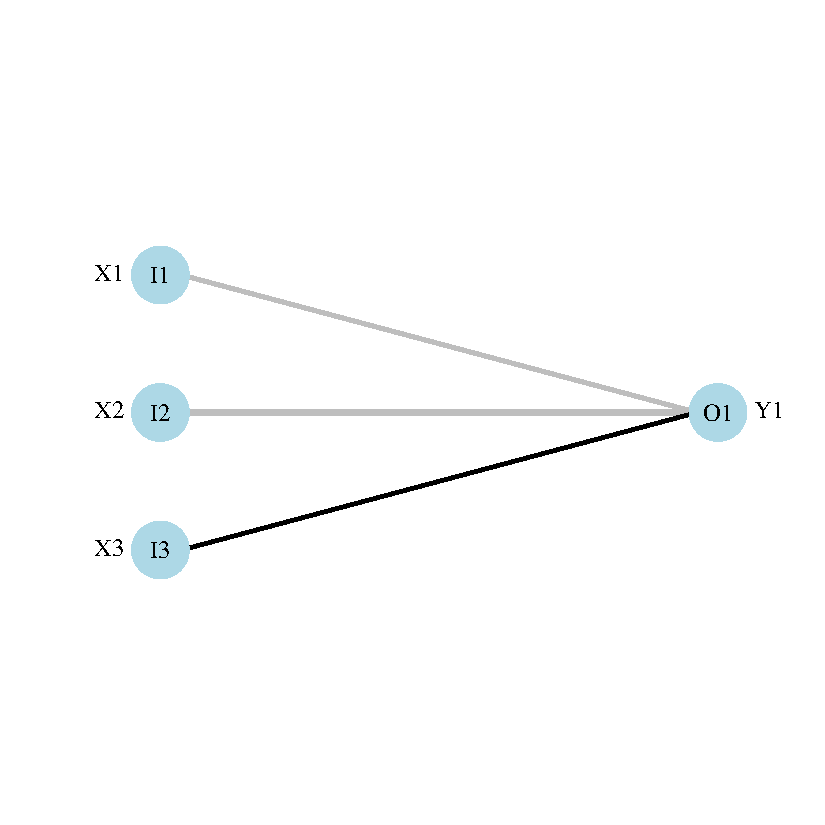
\includegraphics[width=7.5cm,height=7.5cm]{figs/plotnet_skip-1} }
\subfloat[\label{fig:plotnet_skip2}]{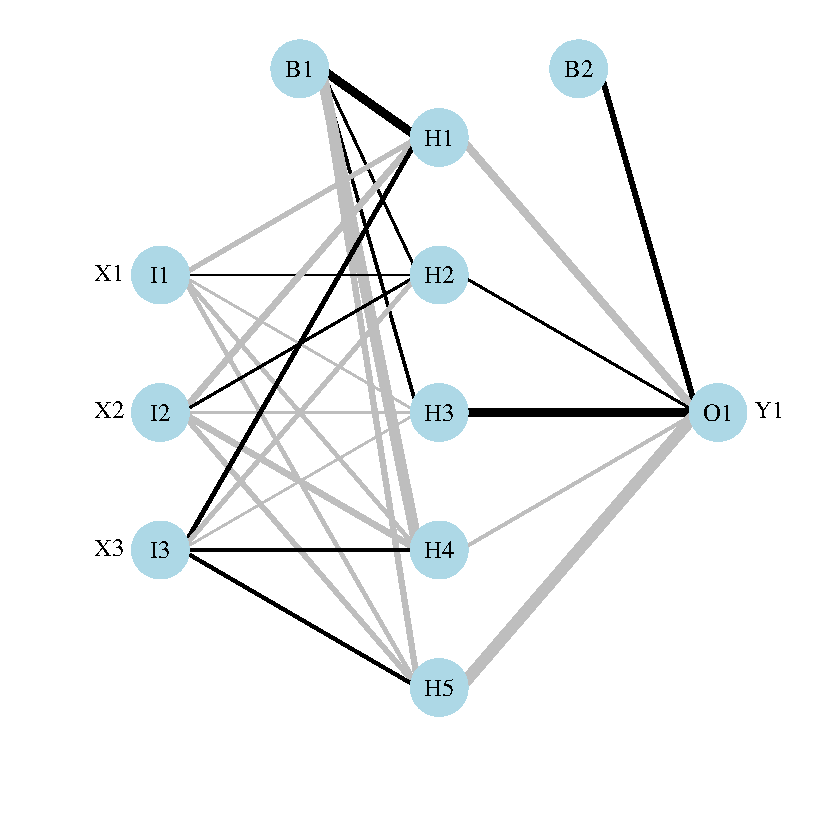
\includegraphics[width=7.5cm,height=7.5cm]{figs/plotnet_skip-2} }

}

\caption{Examples from the \code{plotnet} function showing a neural network with a separate skip layer between the input and output layers.  The skip layer (\ref{fig:plotnet_skip1}) and primary neural network (\ref{fig:plotnet_skip2}) can be viewed separately with \code{plotnet}.}\label{fig:plotnet_skip}
\end{figure}


\end{knitrout}

The \pkg{RSNNS} package provides several algorithms that can be used to prune connections or nodes in a neural network.  This approach can remove connection weights between layers or input nodes that do not contribute to the predictive performance of the network.  Pruning has the benefit of a potential increase in power by increasing the degrees of freedom or the identification of input nodes with low importance.  Algorithms in \pkg{RSNNS} for weight pruning include magnitude based pruning, Optimal Brain Damage, and Optimal Brain Surgeon, whereas algorithms for node pruning include skeletonization and the non-contributing units method \citep{Zell98}.  The \code{plotnet} function can be used to plot a pruned neural network, with options to omit or display the pruned connections (\cref{fig:plotprune}).  

\begin{kframe}
\begin{alltt}
\hlcom{# pruned model using RSNNS}
\hlstd{pruneFuncParams} \hlkwb{<-} \hlkwd{list}\hlstd{(}\hlkwc{max_pr_error_increase} \hlstd{=} \hlnum{10.0}\hlstd{,} \hlkwc{pr_accepted_error} \hlstd{=} \hlnum{1.0}\hlstd{,}
  \hlkwc{no_of_pr_retrain_cycles} \hlstd{=} \hlnum{1000}\hlstd{,} \hlkwc{min_error_to_stop} \hlstd{=} \hlnum{0.01}\hlstd{,}
  \hlkwc{init_matrix_value} \hlstd{=} \hlnum{1e-6}\hlstd{,} \hlkwc{input_pruning} \hlstd{=} \hlnum{TRUE}\hlstd{,} \hlkwc{hidden_pruning} \hlstd{=} \hlnum{TRUE}\hlstd{)}
\hlstd{mod} \hlkwb{<-} \hlkwd{mlp}\hlstd{(x, y,} \hlkwc{size} \hlstd{=} \hlnum{5}\hlstd{,} \hlkwc{pruneFunc} \hlstd{=} \hlstr{"OptimalBrainSurgeon"}\hlstd{,}
 \hlkwc{pruneFuncParams} \hlstd{= pruneFuncParams)}

\hlcom{# plot, pruned connections are omitted (default) or included with prune_col}
\hlkwd{par}\hlstd{(}\hlkwc{mar} \hlstd{=} \hlkwd{c}\hlstd{(}\hlnum{0}\hlstd{,} \hlnum{0}\hlstd{,} \hlnum{0}\hlstd{,} \hlnum{0}\hlstd{))}
\hlkwd{plotnet}\hlstd{(mod,} \hlkwc{rel_rsc} \hlstd{=} \hlkwd{c}\hlstd{(}\hlnum{3}\hlstd{,} \hlnum{8}\hlstd{))}
\hlkwd{plotnet}\hlstd{(mod,} \hlkwc{prune_col} \hlstd{=} \hlstr{'lightblue'}\hlstd{,} \hlkwc{rel_rsc} \hlstd{=} \hlkwd{c}\hlstd{(}\hlnum{3}\hlstd{,} \hlnum{8}\hlstd{))}
\end{alltt}
\end{kframe}\begin{figure}[!ht]

{\centering \subfloat[\label{fig:plotprune1}]{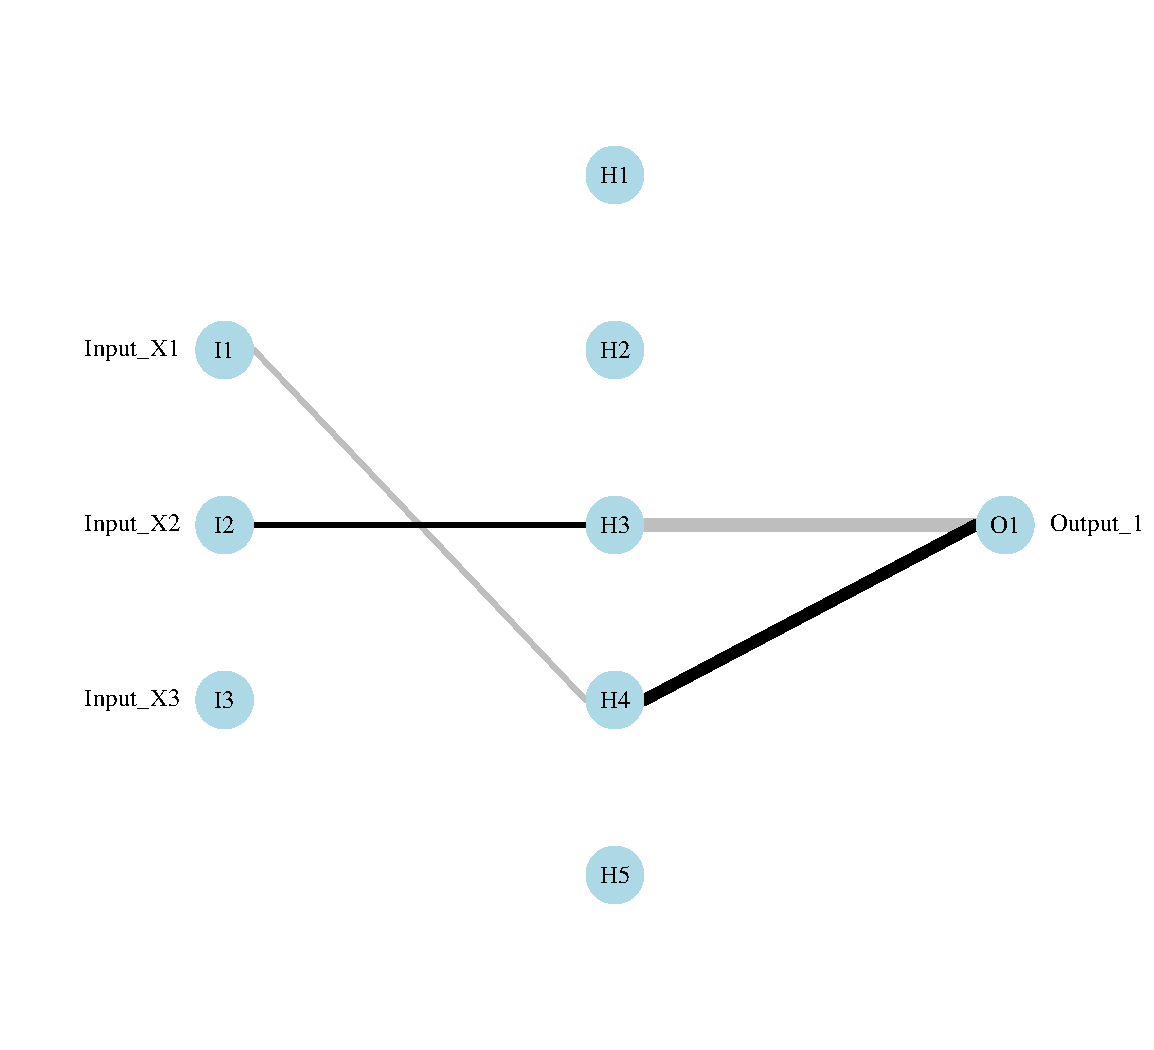
\includegraphics[width=0.48\textwidth]{figs/plotprune-1} }
\subfloat[\label{fig:plotprune2}]{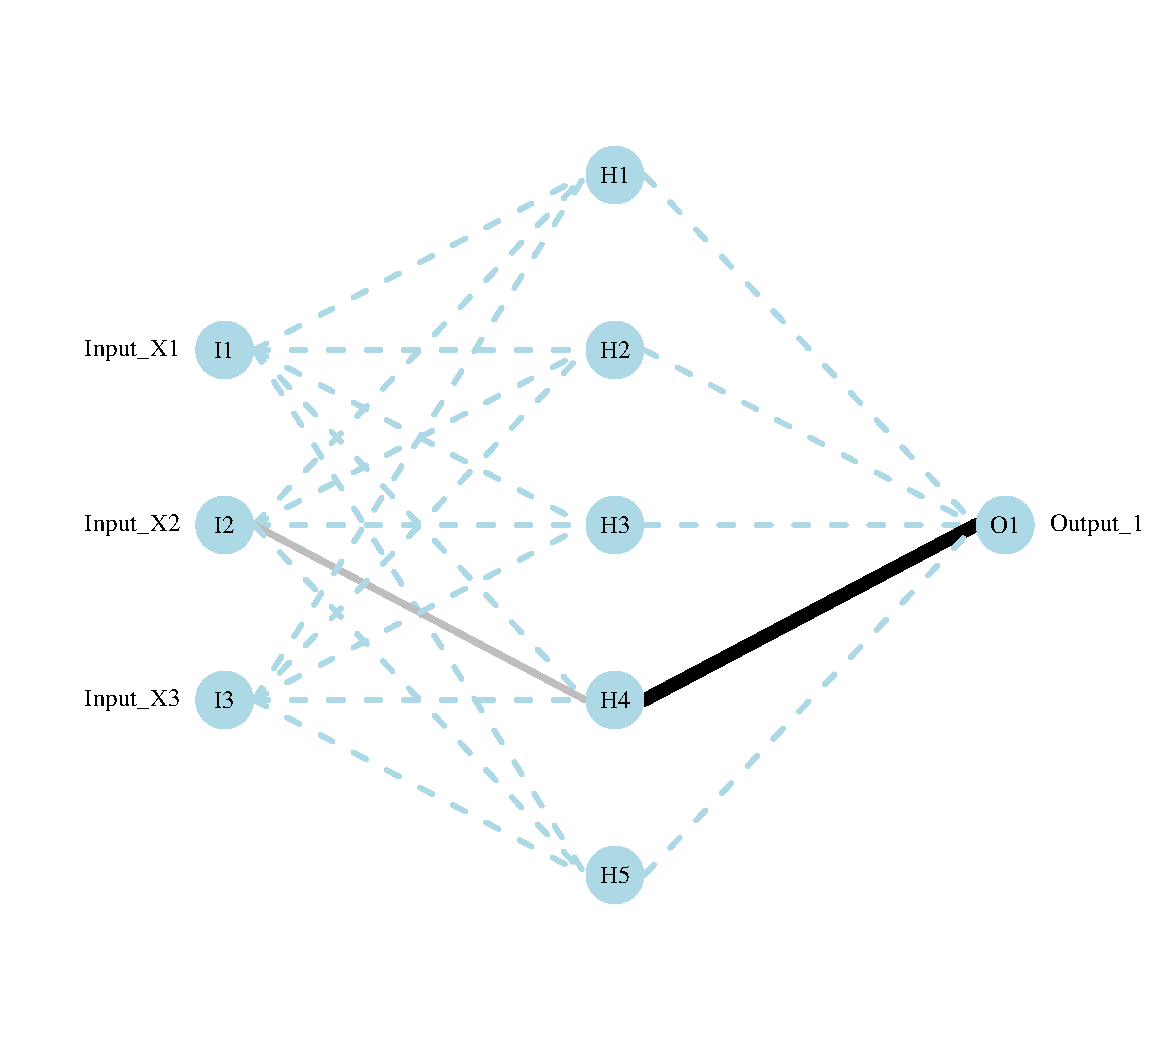
\includegraphics[width=0.48\textwidth]{figs/plotprune-2} }

}

\caption{A pruned neural network using the ``Optimal Brain Surgeon'' algorithm described in \citet{Zell98}.  The default plotting behavior of \code{plotnet} is to omit pruned connections (\ref{fig:plotprune1}), whereas they can be viewed as dashed lines by including the \code{prune\_col} argument (\ref{fig:plotprune2}).}\label{fig:plotprune}
\end{figure}



\subsection{Evaluating variable importance}

The primary benefit of visualizing a \ac{nid} with \code{plotnet} is the ability to evaluate network architecture and the variation in weighted connections between the layers.  Although useful as a general tool, the \ac{nid} is impractical for evaluating most networks given the amount of weighted connections.  Alternative methods to quantitatively describe a neural network deconstruct the model weights to determine variable importance, whereas similar information can only be qualitatively inferred from \code{plotnet}.  Two algorithms for evaluating variable importance are available in \pkg{NeuralNetTools}: Garson's algorithm for relative importance \citep{Garson91,Goh95} and Olden's conection weights algorithm \citep{Olden04}.

Garson's algorithm was originally described by \citet{Garson91} and further modified by \citet{Goh95}.  The \code{garson} function is an implementation of the method described in the appendix of \citet{Goh95}.  This method identifies the relative importance of each variable as an absolute magnitude by deconstructing all weighted connections between the layers in the network. For each input node, all weights connecting an input through the hidden layer to the response variable are identified to return a list of all weights specific to each input variable. A summed product of the connections for each input node are then scaled relative to all other inputs. A value for each input node indicates relative importance as the absolute magnitude from zero to one. The method is limited in that the direction of the response cannot be determined and only neural networks with one hidden layer and one output node can be evaluated.

The \code{olden} function is a more flexible approach to evaluate variable importance using the connection weights algorithm described in \citet{Olden04}. This method calculates importance as the product of the raw input-hidden and hidden-output connection weights between each input and output node and sums the product across all hidden nodes. An advantage is the relative contributions of each connection weight are maintained in both magnitude and sign, as compared to Garson's algorithm which only considers absolute magnitude. For example, connection weights that change sign (e.g., positive to negative) between the input-hidden to hidden-output layers would have a cancelling effect whereas Garson's algorithm may provide misleading results based on the absolute magnitude. An additional advantage is that Olden's algorithm is capable of evaluating neural networks with multiple hidden layers and response variables. The importance values assigned to each variable are also in units based on the summed product of the connection weights, whereas \code{garson} returns importance scaled from 0--1.

Both functions have similar implementations and require only a model object as input.  The default output is a \pkg{ggplot2} bar plot \citep[i.e., \code{geom\_bar},][]{Wickham09} that shows the relative importance of each input variable in the model (\cref{fig:plotimp}).  The plot aesthetics are based on internal code from the function but can be changed using conventional syntax for \pkg{ggplot2}.  The importance values can also be returned as a \code{data.frame} if \code{bar\_plot = FALSE}.  

\begin{kframe}
\begin{alltt}
\hlcom{# garson and olden functions for each model}
\hlkwd{garson}\hlstd{(mod1)}
\hlkwd{olden}\hlstd{(mod1)}
\hlkwd{garson}\hlstd{(mod2)}
\hlkwd{olden}\hlstd{(mod2)}
\hlkwd{garson}\hlstd{(mod3)}
\hlkwd{olden}\hlstd{(mod3)}
\end{alltt}
\end{kframe}

\begin{figure}
\centering
\subfloat[][Model 1 (\code{mlp}), \code{garson}]{


{\centering 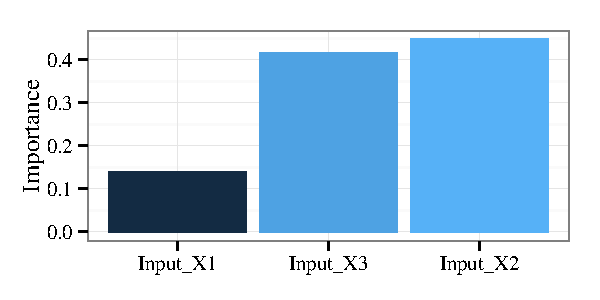
\includegraphics[width=0.47\textwidth]{figs/plotimp-1-1} 

}



\label{fig:plotimp1}
}
\subfloat[][Model 1 (\code{mlp}), \code{olden}]{


{\centering 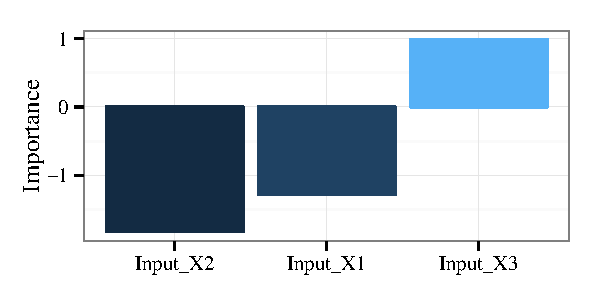
\includegraphics[width=0.47\textwidth]{figs/plotimp-2-1} 

}



\label{fig:plotimp2}
}

\subfloat[][Model 2 (\code{nn}), \code{garson}]{


{\centering 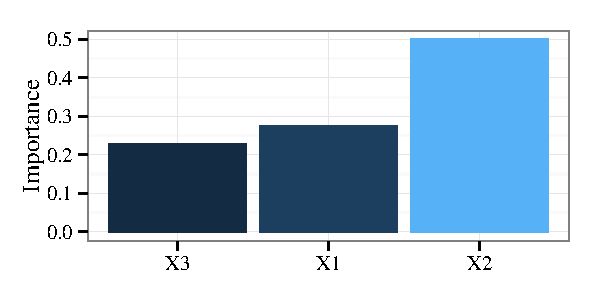
\includegraphics[width=0.47\textwidth]{figs/plotimp-3-1} 

}



\label{fig:plotimp3}
}
\subfloat[][Model 2 (\code{nn}), \code{olden}]{


{\centering 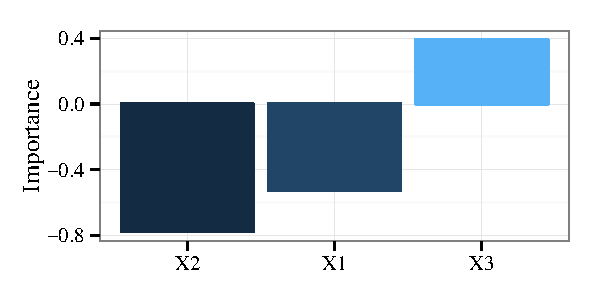
\includegraphics[width=0.47\textwidth]{figs/plotimp-4-1} 

}



\label{fig:plotimp4}
}

\subfloat[][Model 3 (\code{nnet}), \code{garson}]{


{\centering 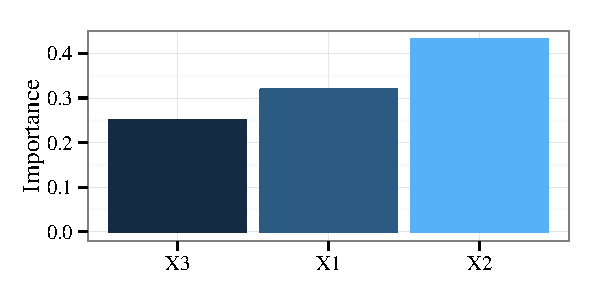
\includegraphics[width=0.47\textwidth]{figs/plotimp-5-1} 

}



\label{fig:plotimp5}
}
\subfloat[][Model 3 (\code{nnet}), \code{olden}]{


{\centering 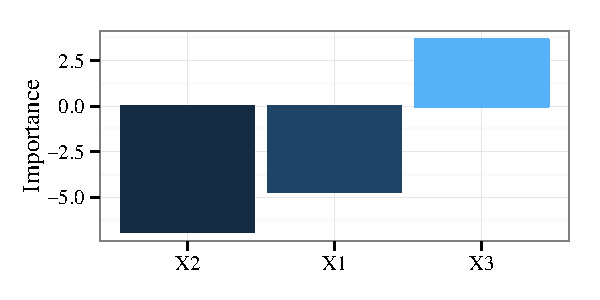
\includegraphics[width=0.47\textwidth]{figs/plotimp-6-1} 

}



\label{fig:plotimp6}
}
\caption{Variable importance for three models using Garson's algorithm for relative importance (\code{garson}, \citealt{Garson91,Goh95}) and Olden's conection weights algorithm (\code{olden}, \citealt{Olden04}).  Garson's algorithm shows importance as absolute values from 0--1 whereas Olden's algorithm preserves sign and magnitude.  Importance values for Olden's algorithm are directly from the summed product of model weights and should only be evaluated based on the sign and relative magnitudes between variables.}
\label{fig:plotimp}
\end{figure}

\subsection{Sensitivity analysis}

An alternative approach to evaluate variable interactions in a neural network is the Lek profile method, described briefly in \citet{Lek96} and in more detail in \citet{Gevrey03}. The profile method is fairly generic and can be extended to any statistical model in \pkg{R} with a \code{predict} method. However, it is one of few methods used to evaluate sensitivity in neural networks.  The profile method differs fundamentally from the variable importance algorithms by evaluating the behavior of response variables across different values of the input variables.  

The \code{lekprofile} function evaluates the effect of explanatory variables by returning a plot of the predicted response across the range of values for each variable.  A critical aspect of the method is the remaining explanatory variables that are held constant when separately evaluating each input variable.  The \code{lekprofile} function provides two options for determining constant values of unevaluated explanatory variables.  The first option following the original profile method evaluates effects of each variable while holding the remaining expalanatory variables at different quantiles (e.g., minimum, 20th percentile, maximum, \cref{fig:plotlek_sens1,fig:plotlek_bars1}). This is implemented by creating a matrix of values for explanatory variables where the number of rows is the number of observations in the original dataset and the number of columns is the number of explanatory variables. All explanatory variables are held at their median (or other constant value), while the variable of interest is sequenced from its minimum to maximum value across the range of observations. This matrix is then used to predict values of the response variable from a fitted model object. This is repeated for each explanatory variable to obtain all response curves.  Constant values are defined by passing one or more numeric values in the range 0--1 to the \code{group\_vals} that define the quantiles, with the default as minimum, 20\textsuperscript{th}, 40\textsuperscript{th}, 60\textsuperscript{th}, 80\textsuperscript{th}, and maximum percentiles.  

An alternative implementation of \code{lekprofile} is to group the unevaluated explanatory variables using natural groupings defined by statistical properties of the data. Covariance among predictors may present unlikely scenarios if all unevaluated variables at held at the same level (e.g., high values for one variable may be unlikely to co-occur with high values for a second variable). To address this issue, a second option is available to hold unevaluated variables at mean values defined by natural clusters in the data (\cref{fig:plotlek_sens2,fig:plotlek_bars2}). Clusters are identified using {\it k}-means clustering (\code{kmeans} from base \pkg{stats}, \citealt{Hartigan79}) of the input variables if the argument passed to \code{group_vals} is an integer value greater than one. The centers (means) of the clusters are then used as constant values for the unevaluated variables.  \citet{Beck14a} provide an example of the clustering method for \code{lekprofile} by evaluating response of a lake health index to different explanatory variables.  Lake clusters were identified given covariance among explanatory variables, such that holding explanatory variables at related values created more ecologically relevant response curves.  Similar plots can be created with \code{lekprofile} as response curves (\cref{fig:plotlek_sens}) or to visualize the groupings for unevaluated explanatory variables (\cref{fig:plotlek_bars}).  For the latter case, \code{split\_show = TRUE} will return a stacked bar plot for each group with heights in each bar proportional to the constant values.
\begin{kframe}
\begin{alltt}
\hlcom{# lek profile, quantile evaluation}
\hlkwd{lekprofile}\hlstd{(mod3)}

\hlcom{# lek profile, quantile groups }
\hlkwd{lekprofile}\hlstd{(mod3,} \hlkwc{group_show} \hlstd{=} \hlnum{TRUE}\hlstd{)}

\hlcom{# lek profile, cluster evaluation}
\hlkwd{lekprofile}\hlstd{(mod3,} \hlkwc{group_vals} \hlstd{=} \hlnum{6}\hlstd{)}

\hlcom{# lek profile, cluster groups}
\hlkwd{lekprofile}\hlstd{(mod3,} \hlkwc{group_vals} \hlstd{=} \hlnum{6}\hlstd{,} \hlkwc{group_show} \hlstd{=} \hlnum{TRUE}\hlstd{)}
\end{alltt}
\end{kframe}

\begin{figure}
\centering
\subfloat[][Response with quantiles]{


{\centering 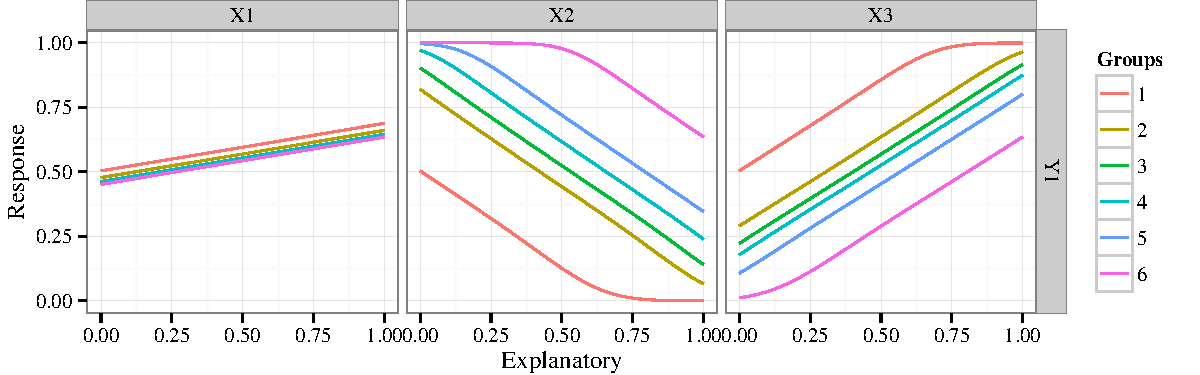
\includegraphics[width=0.9\textwidth]{figs/plotlek_sens1-1} 

}



\label{fig:plotlek_sens1}
}

\subfloat[][Response with clusters]{


{\centering 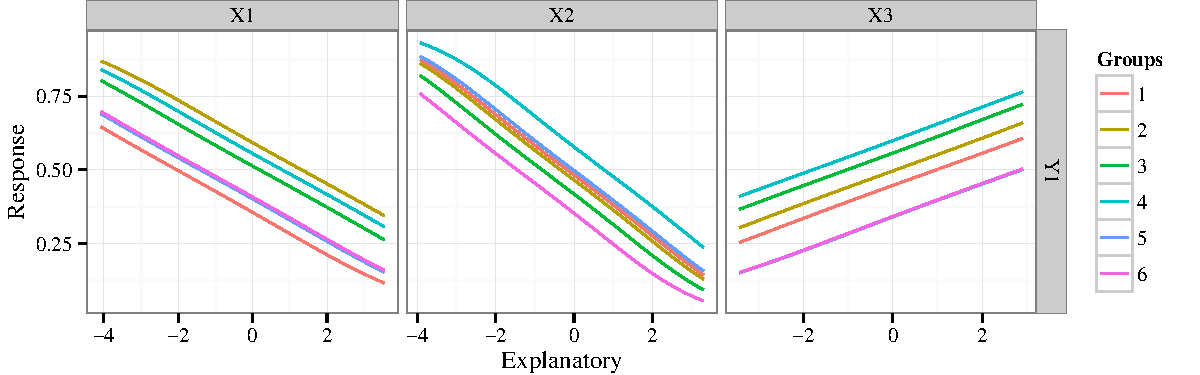
\includegraphics[width=0.9\textwidth]{figs/plotlek_sens2-1} 

}



\label{fig:plotlek_sens2}
}s
\caption{Sensitivity analysis ofa  neural network using the Lek profile method to evaluate the effects of explanatory variables.  \Cref{fig:plotlek_sens1} groups unevaluated explanatory variables at quantiles and \cref{fig:plotlek_sens2} groups by cluster means from {\it k}-means clustering of all explanatory variables.  Values at which explanatory variables are held constant in each plot are shown in \cref{fig:plotlek_bars1,fig:plotlek_bars2}, respectively.}
\label{fig:plotlek_sens}
\end{figure}

%%%%
\begin{figure}
\centering
\subfloat[][Quantile groupings]{


{\centering 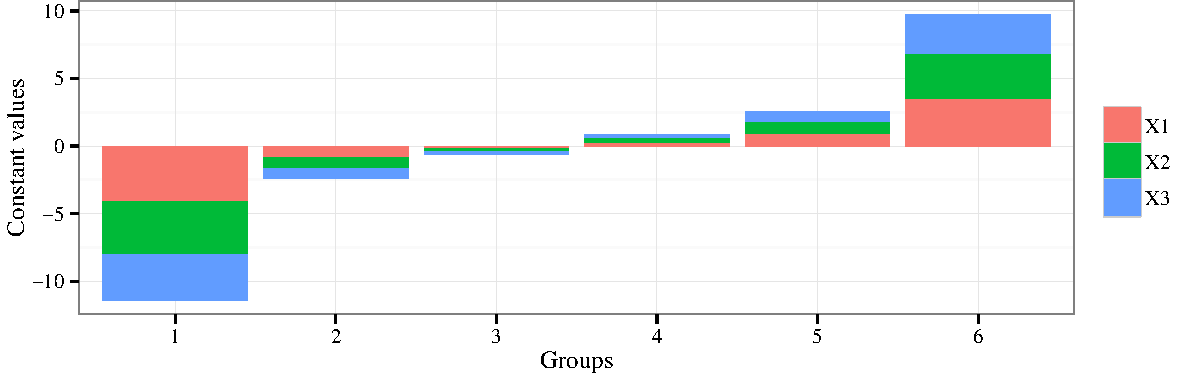
\includegraphics[width=0.9\textwidth]{figs/plotlek_bars1-1} 

}



\label{fig:plotlek_bars1}
}

\subfloat[][Cluster groupings]{


{\centering 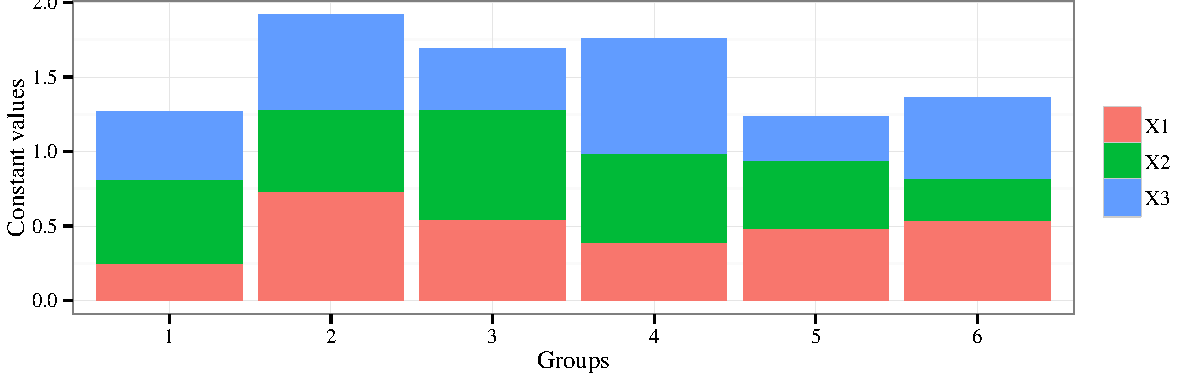
\includegraphics[width=0.9\textwidth]{figs/plotlek_bars2-1} 

}



\label{fig:plotlek_bars2}
}
\caption{Bar plots for values in each group of unevaluated explanatory variables in \cref{fig:plotlek_sens1,fig:plotlek_sens2}.  \Cref{fig:plotlek_bars1} shows default quantile groupings set at the minimum, 20\textsuperscript{th}, 40\textsuperscript{th}, 60\textsuperscript{th}, 80\textsuperscript{th}, and maximum percentiles.  For example, variables are held at zero for group 1 (i.e., stacked bars with no height) for the minimum value, whereas group 6 holds variables at their maximum of one. \Cref{fig:plotlek_bars2} shows the cluster centers for each variable in each group identified from {\it k}-means clustering.}
\label{fig:plotlek_bars}
\end{figure}

\section[Applied example]{Applied example}

Although \pkg{NeuralnetTools} provides several methods to extract information from a neural network, it does not provide explicit guidance for developing the initial model.  A potentially more challenging aspect of using neural netwworks is understanding the effects of network architecture, appropriate use of training and validation datasets, and implications for the bias-variance tradeoff with model over- or under-fitting during model development.  A detailed discussion of these issues is beyond the scope of this paper, although an example application is presented below to introduce a `best practices' approach to model development.  The models presented above, including the \code{neuraldat} dataset, are contrived examples to illustrate use of the \pkg{NeuralNetTools} package and they do not demonstrate a comprehensive application of neural networks in practice.  Several texts provide explicit guidelines on developing neural network models \cite[e.g.,][]{Ripley96, Lek00, Maier00}.  In general, the following should be considered during model development:
\begin{itemize}
\item Initial data pre-processing to normalize inputs and standardize response,
\item Network architecture including number of hidden layers, number of nodes in each hidden layer, inclusion of bias or skip layers, pruning weights or inputs,
\item Split of dataset into a training and test dataset, e.g., 2:1, 3:1, leave-one-out, etc., 
\item Initial starting weights for the back-propagation algorithm, and
\item Criteria for stopping model training iterations, e.g., error convergance tolerance, maximum number of iterations, minimum error on test dataset, etc.
\end{itemize}

A dataset from the \pkg{nycflights13} package \citep{Wickham14b} is used to demonstrate the effects of different training methods on model conclusions.  This dataset describes flight data for all flights departing New York City (i.e., JFK, LGA, or EWR) in 2013.  The example focuses on all flights from the `UA' carrier in the month of December to identify variables that potentially influence arrival delays (\code{arr\_delay}) at the destination airport.  Factors potentially related to delays were selected from the dataset and included departure delay (\code{dep\_delay}), departure time (\code{dep\_time}), arrival time (\code{arr\_time}), travel time between desinations (\code{air\_time}), and distance flown (\code{distance}).  All explanatory variables are normalized and the response variable is standardized to 0--1.  

The effects of network architecture and initial starting weights on indications of variable importance were evaluated by creating a large number of models and assessing the uncertainty of the importance measures.  Models with one, five, or ten hidden nodes and 100 separate models for each node level with a different set of random starting weights were evaluated.  The relative importance of the variables was saved for each model and combined in a single plot to show overall variable importance as the median and 5\textsuperscript{th}/95\textsuperscript{th} percentiles from the 100 models for each node level (get \href{code}{}). 

Several conclusions about the dataset and effects of network architecture can be made from the results in \cref{fig:flightimp}.  First, delays in arrival time are consistently negatively related to distance travelled and positively related to departure delays and time in the air.  That is, flights arrived later than their scheduled destination time if flight time was long or if their departure was delayed, whereas flights arrived earlier than scheduled for longer distances.  Second, the indications of importance varied in the range of magnitude between the models (i.e., one node  varied +/- 1 and the others +/- 3).  This result suggests that the absolute values of importance only have relevance within a model, whereas only the relative rankings (e.g., least, most important) can be compared between models.  Third and most important, the level of uncertainty for specific variables can be large between model fits for the same architecture (i.e., effect of random starting weights).  This conclusion emphasizes that a single model can often provide misleading information about variable importance such that several fits are often required before results are stabilized.  Additional considerations described above (e.g., criteria for stopping training, use of training and test datasets) can also affect conclusions of variable importance and should be equally considered during model development.


\begin{figure}
\centering
\subfloat[][Networks with one node]{


{\centering 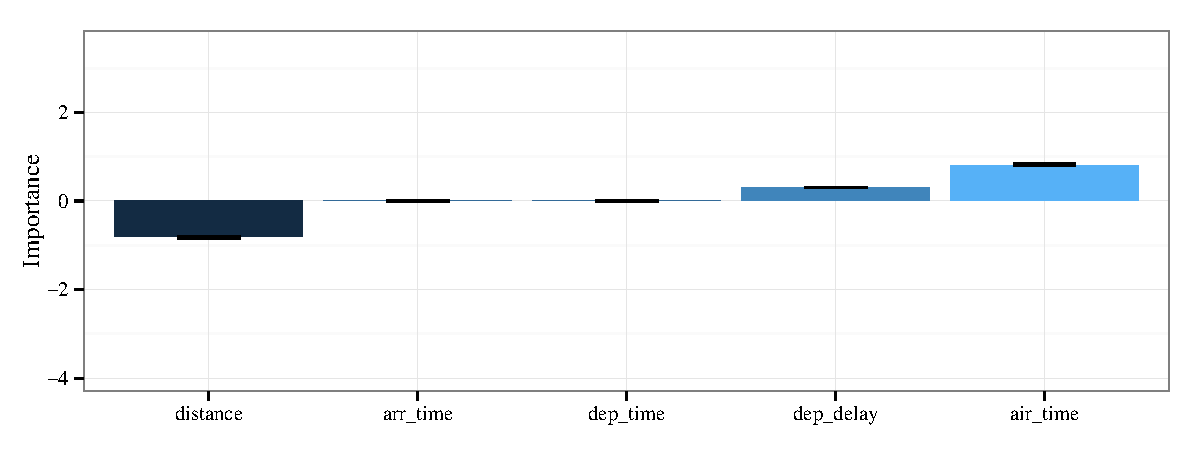
\includegraphics[width=0.95\textwidth]{figs/flightimp-1-1} 

}



\label{fig:flightimp1}
}

\subfloat[][Networks with five nodes]{


{\centering 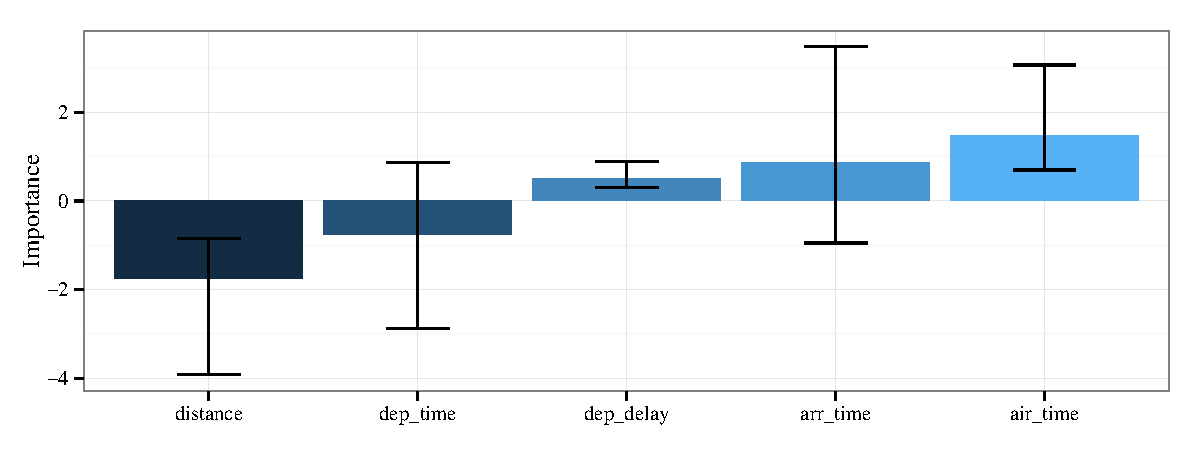
\includegraphics[width=0.95\textwidth]{figs/flightimp-2-1} 

}



\label{fig:flightimp2}
}

\subfloat[][Networks with ten nodes]{


{\centering 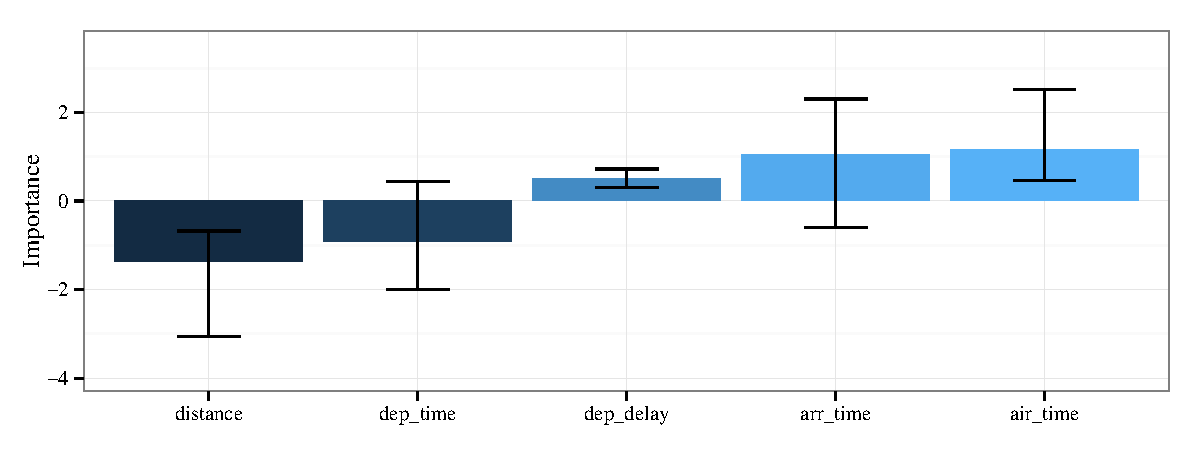
\includegraphics[width=0.95\textwidth]{figs/flightimp-3-1} 

}



\label{fig:flightimp3}
}
\caption{Uncertainty in variable importance estimates for three neural networks to evaluate factors related to arrival delays for flights departing New York City.  Three model types with one, five, and ten nodes were evaluated with 100 models with different starting weights for each type.}
\label{fig:flightimp}
\end{figure}

\section[Conclusions]{Conclusions}

The \pkg{NeuralNetTools} package provides a simple approach that improves the quality of information obtained from a feed-forward \ac{mlp} neural network.  Functions in the package can be used to visualize a neural network using a \acl{nid} (\code{plotnet}), evaluate variable importance (\code{garson}, \code{olden}), and conduct a sensitivity analysis (\code{lekprofile}).  Methods are available for the most used \ac{CRAN} packages that can create neural networks (\pkg{caret}, \pkg{neuralnet}, \pkg{nnet}, \pkg{RSNNS}), whereas additional methods will be made available based on future popularity of the remaining packages (\pkg{AMORE}, \pkg{FCNN4R}, \pkg{monmlp}, \pkg{qrnn}).  A primary objective of the package is to dispel the myth that supervised neural networks for prediction are `black boxes' that provide no information about underlying relationships between the variables \citep{Paruelo97,Olden02}.  Although neural networks are considered complex relative to more conventional approaches, the theoretical foundation has many parallels with traditional modelling techniques that can allow insight into causation.  Moreover, the model fitting process requires the minimization of an objective function such that conventional techniques to evaluate model sensitivity or performance (e.g., cross-validation) can be used with neural networks.  Functions in \pkg{NeuralNetTools} can facilitate the selection of the optimal network architecture or can be used for post-hoc assessment. 

A more compelling issue is when and how to apply neural networks given alternative methods for data-intensive exploration.  The popularity of the \ac{mlp} neural network is partially the cause of misperceptions and generalizations of their benefits as modelling tools \citep{Burke97}. Indeed, the `neural' component of neural networks is advertised as a mathematical representation of the network of synaptic impulses in the human brain, although the former is of course an over-simplification of the latter.  Several examples have shown that the \ac{mlp} network may provide comparable predictive performance as similar statistical methods \citep{Feng02,Razi05,Beck14a}.  As such, the neural network should be considered a tool in the larger toolbox of data-intensive methods that should be used after examination of the tradeoffs between techniques, with particular emphasis on the needs of a given dataset or research question.  For example, an appropriate method should be chosen based on power given the sample size, expected linear or non-linear interactions between variables, distributional forms of the response, and other relevant concerns that are routinely considered during exploratory data analysis.  The true value of the \pkg{NeuralNetTools} package is a set of analysis tools that can inform a more balanced assessment given the alternative and complementary methods for data-intensive exploration.

\section[Acknowledgments]{Acknowledgments}
 
I would like to thank Bruce Vondracek, Sanford Weisberg, and Bruce Wilson of the University of Minnesota for general guidance during the development of this package.  Contributions and suggestions from online users have also greatly improved the utility of the package.    

% note that ref titles need to be in title-case 
\bibliographystyle{jss}
\bibliography{refs}

\end{document}
